\labsection{ПРИЛОЖЕНИЯ}

\labsection{Газовый разряд}

Под термином <<газовый разряд>> обычно понимают все явления и процессы, связанные с протеканием электрического тока
через газ.

Само название \important{разряд} произошло от названия медленно протекающего процесса потери заряда заряженными металлическими
телами, расположенными на подставке из изолятора, что наблюдалось ещё в XVI~веке. Позднее Кулон экспериментально
доказал, что заряд стекает с проводника через воздух, а не через подставку из изолятора, то есть по современной
терминологии имеет место газовый разряд. Разряд при низких давлениях воздуха (порядка 1~мбар) открыл и исследовал
Фарадей~--- этот разряд стал известен как \important{тлеющий}. В конце XIX~века исследование проводимости разреженных газов
привело Дж.Дж.~Томсона к открытию первой элементарной частицы~--- электрона, а дальнейшие исследования физики газового
разряда во многом послужили экспериментальной основой атомной и квантовой физики.

Основателем физики собственно газового разряда считается Таунсенд, ученик Дж.~Дж.~Томсона, создавший в начале XX~века
теорию пробоя газа и установивший закономерности ионизации. Следующий принципиальный вклад в физику газового разряда был
внесён Ленгмюром, который вместе с Тонксом в 1928~году, исследуя газовый разряд низкого давления, ввёл такое
фундаментальное понятие физики, как плазма, о чём уже говорилось выше, а также развил методы исследования плазмы, в
частности, метод зондов.

Современная физика термин \important{газовый разряд} трактует в более широком смысле. Это~--- не только процесс протекания
тока через газ, но и любой процесс возникновения ионизации газа под действием приложенного электрического поля. При этом
поле может быть не только постоянным во времени, но и быстропеременным~--- высокочастотным (ВЧ-разряд, мегагерцы),
сверхвысокочастотным (СВЧ-разряд, гигагерцы) и даже оптического диапазона (оптический разряд). В последнее время был
открыт пучково-плазменный разряд (ППР), загорающийся при прохождении электронного пучка через газ малой плотности
вследствие возникновения в такой системе плазменных колебаний СВЧ-диапазона. Термины \important{гореть, зажигание}
получили распространение потому, что при возникновении достаточно сильной ионизации газ светится.

Разряды в постоянном поле разделяют на \important{несамостоятельные} и \important{самостоятельные}. Дело в том, что при нормальных
условиях газы состоят в основном только из электрически нейтральных атомов и молекул и, по сути, являются диэлектриками,
то есть изоляторами, поэтому через них не может проходить сколько-нибудь заметный электрический ток. Проводниками могут
быть только хоть в какой-то мере ионизованные газы, то есть газы, содержащие свободные заряды~--- носители тока. В газах
это~--- положительные и отрицательные ионы и электроны. Ионы в газах могут возникать в результате действия различных
ионизаторов, например, ультрафиолетового излучения или рентгеновских лучей, космического излучения, лучей радиоактивных
загрязнений, столкновений атомов газа с электронами и другими частицами, энергия которых превышает потенциал ионизации
атомов газа.

Предположим, что ионы в газовом проводнике создаются исключительно внешним ионизатором. Тогда при прекращении действия
этого ионизатора ток и, следовательно, разряд прекращаются. Такой разряд называется несамостоятельным.
\todo[author = Andrew]{В картинке для нанесения некоторых обозначений был использован psfrag, который несовместим с pdf. Необходимо исправить изображение.}

\begin{figure}[h!]
	\centering
	\psfrag{u}{$U$}
	\psfrag{i}{$I$}
	\psfrag{0}[rt]{0}
	\psfrag{a}[br]{А}
	\psfrag{b}{Б}
	\psfrag{v}{В}
	\psfrag{g}{Г}
	\psfrag{d}{Д}
	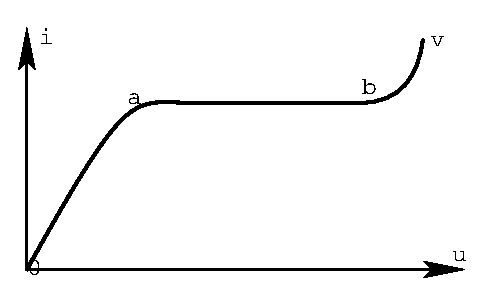
\includegraphics[width=0.7\textwidth]{Chapter_5/v5_2}
	\caption{Вольт-амперная характеристика несамостоятельного газового разряда}
	\figmark{Non-self discharge VAC}
\end{figure}

Типичная кривая, отображающая связь между током через газовый промежуток и напряжением на нём для несамостоятельного разряда показана на рис.~\figref{Non-self discharge VAC}. С повышением напряжения
на газовом промежутке ток сначала возрастает (кривая ОА), а потом достигает насыщения и остаётся практически постоянным (участок АБ), что соответствует полному вытягиванию на электроды зарядов, создаваемых внешним ионизатором.

При дальнейшем повышении напряжения ток снова начинает возрастать (участок БВ). Это значит, что имеющиеся ионы, и прежде всего электроны, за период между двумя последовательными столкновениями набирают такую энергию, что возникнет
\important{столкновительная ионизация}, то есть рождение новых, \important{вторичных ионов}. При этом возникают и развиваются
\important{электронные лавины}. Итак, мы будем иметь дело с \important{размножением,} или усилением, часто называемым \important{газовым
усилением}. При каком значении поля наступит размножение, зависит от давления газа и энергии, необходимой для ионизации
данной молекулы (потенциала ионизации). В результате усиления концентрация ионов возрастает до величины, которая линейно
или даже более сильно зависит от первичной ионизации. При этом разряд остаётся несамостоятельным.

Однако в достаточно сильном электрическом поле проводимость газа может возрасти скачком~--- возникает \important{пробой}.
Соответствующее напряжение на газовом промежутке называется \important{напряжением пробоя}, или \important{напряжением зажигания}.
Если после возникновения пробоя убрать внешний ионизатор, то разряд не прекращается. Разряд перешёл в \important{режим
самостоятельного разряда}: теперь ионизация поддерживается процессами в самом разряде.
\todo[author = Andrew]{В картинке для нанесения некоторых обозначений был использован psfrag, который несовместим с pdf. Необходимо исправить изображение.}

\begin{figure}[h!]
	\centering
	\psfrag{0}{0}
	\psfrag{a}[rb]{$x$}
	\psfrag{D}[cb]{$dx$}
	\psfrag{d}[rb]{$d$}
	\psfrag{x}{$X$}
	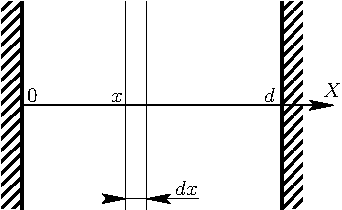
\includegraphics[width=0.7\textwidth]{Chapter_5/v5_3}
	\caption{К выводу критерия Таунсенда}
	\figmark{Townsend criterion}
\end{figure}


Как уже было сказано, первая модель перехода несамостоятельного разряда в самостоятельный была предложена Таунсендом.
Следуя Таунсенду, введём \important{коэффициент объёмной ионизации} $\alpha$, численно равный количеству электронно-ионных
пар, образуемых одним электроном на единице длины пути. По смыслу ясно, что этот коэффициент зависит от давления
(возрастает с увеличением числа соударений, то есть с давлением) и от напряжённости электрического поля $E$ (возрастает
с полем).

Рассмотрим, как происходит ионизация в газовом промежутке между плоскими электродами~--- катодом и анодом (рис.~\figref{Townsend criterion}). На
расстоянии~$x$ от катода в слое толщины $dx$ один электрон создаёт $\alpha dx$ пар ионов. Если со стороны катода в этот
слой втекает электронный ток $I_e$, то в слое он возрастёт на величину $dI_e=I_e\alpha dx$. Интегрирование этого
уравнения в предположении, что $\alpha$ не зависит от $x$ (то есть поле не зависит от $x$, что верно только при малых
токах, когда нет объёмных зарядов), даёт
\begin{equation*}
	I_e(x)=I_e(0)e^{\alpha x},
\end{equation*}
где $I_e(0)$~--- электронный ток, втекающий с катода в газовый промежуток. Можно видеть, что на аноде, то есть
при $x=d$, он возрастает в $e^{\alpha d}$~раз. Например, при $\alpha=3~\text{см}^{-1}$ и $d=3$~см ток возрастёт приблизительно
на 4 порядка. Это и есть режим газового усиления, то есть размножения электронно-ионных пар вследствие развития
электронных лавин. Однако при этом разряд ещё не обязательно переходит в режим самостоятельного. Например, если ток
$I_e(0)$ создаётся только внешним ионизатором, то при его выключении прекращается и ток через промежуток. Чтобы разряд
не прекращался, нужно, чтобы ток $I_e(0)$ поддерживался самим разрядом, то есть чтобы образовалась положительная
обратная связь. Такая связь может установиться только через поток частиц, двигающихся из разряда в обратном направлении,
к катоду. В модели Таунсенда это~--- положительные ионы и фотоны. Далее будем учитывать только положительные ионы.

Полный ток через любое поперечное сечение разряда $x=const$ один и тот же и складывается из тока, переносимого
электронами, и тока, переносимого движущимися навстречу им положительными ионами. Следовательно, полный ток на аноде
равен чисто электронному току $I_e(d)$, а ионный ток на катоде $I_i(0)$ равен
\begin{equation*}
	I_i(0)=I_e(d)-I_e(0)=I_e(0)(e^{\alpha d}-1).
\end{equation*}

Пусть теперь каждый пришедший на катод ион выбивает из катода в среднем $\gamma$ вторичных электронов ($\gamma$~--- коэффициент вторичной ионно-электронной эмиссии, $\gamma=10^{-1}-10^{-3})$. Тогда из катода пойдёт ток этих вторичных электронов $I_2$:
\begin{equation*}
	I_2=\gamma I_i(0)=\gamma I_e(0)(e^{\alpha d}-1),
\end{equation*}
а полный электронный ток из катода будет складываться из тока $I_1$, образуемого внешним ионизатором, и тока вторичных
электронов $I_2$:
\begin{equation*}
	I_e(0)=I_1+I_2=I_1+\gamma I_e(0)(e^{\alpha d}-1),
\end{equation*}
так что
\begin{equation*}
	I_e(0)=\frac{I_1}{1-\gamma(e^{\alpha d}-1)}.
\end{equation*}

Таким образом, полный ток через газовый промежуток $I_i$, равный электронному току через анод, будет равен
\begin{equation*}
	I_i=I_e(d)=I_e(0)e^{\alpha d}=\frac{I_1e^{\alpha d}}{1-\gamma(e^{\alpha d}-1)}.
\end{equation*}

С повышением напряжения на газовом промежутке, то есть с ростом электрического поля, растут коэффициенты $\alpha$ и
$\gamma$, и ток возрастает. Разряд тем не менее остаётся несамостоятельным, так как при выключении внешнего ионизатора
($I_1=0$) ток обращается в нуль. Однако при достижении некоторого значения поля знаменатель этого выражения обратится в
нуль, а ток~--- в бесконечность при любом сколь угодно малом значении $I_1$, так что внешний ионизатор можно вообще
убрать. Это и есть \important{переход от несамостоятельного разряда к самостоятельному}, или \important{наступление пробоя}, а его
условие~--- \important{критерий Таунсенда}, следовательно, имеет вид
\begin{equation*}
	\gamma(e^{\alpha d}-1)=1.
\end{equation*}
Величина
\begin{equation*}
	\mu\equiv\gamma(e^{\alpha d}-1)
\end{equation*}
называется \important{коэффициентом воспроизводства}, поскольку она показывает, сколько электронов воспроизводится на катоде в
результате прохождения через разряд одного электрона, вышедшего с катода.
\todo[author = Andrew]{В картинке для нанесения некоторых обозначений был использован psfrag, который несовместим с pdf. Необходимо исправить изображение.}

\begin{figure}[h!]
	\centering
	\psfrag{P}[rb]{$P\.d$, см\.Торр}
	\psfrag{V}[lb]{$U_з$, В}
	\psfrag{2}[tc]{\footnotesize2}
	\psfrag{4}[tc]{\footnotesize4}
	\psfrag{6}[tc]{\footnotesize6}
	\psfrag{a}[tc]{\small$10^{-1}$}
	\psfrag{b}[tc]{\small$10^0$}
	\psfrag{c}[tc]{\small$10^1$}
	\psfrag{d}[tc]{\small$10^2$}
	\psfrag{e}[tc]{\small$10^3$}
	\psfrag{A}[rc]{\small$10^2$}
	\psfrag{B}[rc]{\small$10^3$}
	\psfrag{C}[rc]{\small$10^4$}
	\psfrag{3}[rc]{\footnotesize2}
	\psfrag{5}[rc]{\footnotesize4}
	\psfrag{7}[rc]{\footnotesize6}
	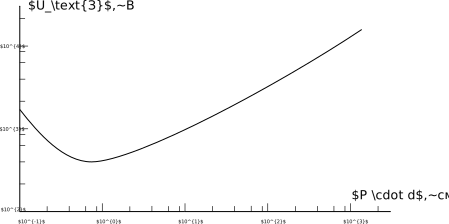
\includegraphics[width=0.7\textwidth]{Chapter_5/v5_4}
	\caption{Зависимость потенциала зажигания $U_\text{з}$ от произведения давления~$P$ на~длину $d$ разрядного промежутка (кривая Пашена) для воздуха}
	\figmark{Paschen curve}
\end{figure}

	
Зная функции $\gamma(E)$ и $\alpha(E)$, из этого условия можно определить пробивающее поле, пробивное напряжение или, в
случае разряда, \important{потенциал зажигания} $U_\text{з}$. Эта теория хорошо подтверждает экспериментально установленный
\important{закон Пашена}, согласно которому потенциал зажигания зависит только от произведения давления на длину разрядного
промежутка, причём эта зависимость имеет минимум (рис.~\figref{Paschen curve}). Таким образом, для заданного давления имеется такая длина
разрядного промежутка, при которой потенциал зажигания и соответствующее ему поле минимальны. Напомним, что в модели
Таунсенда поле в промежутке однородно и не искажается объёмными зарядами, что верно только для разряда с очень маленьким
током. Такой самостоятельный разряд известен как \important{тёмный таунсендовский разряд}. Описанный процесс пробоя также
называют таунсендовским. В газах высокого давления (больше атмосферного) и при больших длинах промежутков реализуется
другой механизм пробоя~--- \important{стриммерный}, или \important{искровой}, а возникающий в результате такого пробоя
нестационарный разряд известен как \important{искровой}. Примером такого разряда является молния.

В широком смысле термин \important{электрический пробой} означает превращение изолятора в проводник в результате приложения к
нему достаточно сильного поля. Для газа это означает переход в ионизованное состояние. При этом возрастание тока
приводит к ещё большему возрастанию концентрации ионов, что приводит к возрастанию проводимости и, следовательно, к
понижению напряжения, необходимого для поддержания такого тока. Если ввести понятие \important{дифференциальное
сопротивление} как производную по току от напряжения, то в этом случае возникает новое явление~--- \important{отрицательное
дифференциальное сопротивление}. Напомним, что для проводников, подчиняющихся закону Ома, например металлов,
дифференциальное сопротивление просто равно обычному сопротивлению и всегда положительно.

Будем и далее характеризовать электрические свойства газового промежутка, заключённого между двумя помещёнными в газ
электродами, вольт-амперной характеристикой (ВАХ). Так принято делать всегда в случае нелинейной зависимости тока через
проводящий элемент от приложенного напряжения.

Экспериментально ВАХ газового проводника~--- например, промежутка между двумя электродами, помещёнными в стеклянную
трубку, заполненную газом,~--- снимают с помощью схемы, представленной на рис.~\figref{Gas gap VAC scheme}. Цепь содержит источник постоянного
напряжения $E$, величину которого можно изменять в пределах примерно от 100~В до нескольких кВ, и переменное
сопротивление $R$, называемое балластным, или нагрузочным. Это сопротивление необходимо для ограничения тока в цепи и
стабилизации разряда на участках с отрицательным дифференциальным сопротивлением. Дело в том, что на этих участках
разряд неустойчив и ток имеет тенденцию неограниченно нарастать. Можно показать, что для устойчивости разряда сумма
отрицательного и положительного сопротивлений такой цепи должна быть положительной, то есть в точке пересечения с ВАХ
нагрузочная прямая должна иметь больший наклон, чем участок кривой ВАХ (рис.~\figref{Neon discharge VAC}).
\todo[author = Andrew]{В картинке для нанесения некоторых обозначений был использован psfrag, который несовместим с pdf. Необходимо исправить изображение.}

\begin{figure}[h!]
	\centering
	\psfrag{A}[cc]{$A$}
	\psfrag{V}[cc]{$V$}
	\psfrag{R}{$R$}
	\psfrag{E}[cb]{$\E$}
	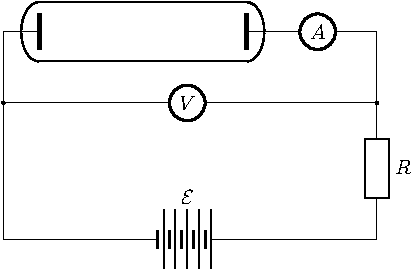
\includegraphics[width=0.7\textwidth]{Chapter_5/v5_5}
	\caption{Схема для снятия ВАХ газового промежутка}
	\figmark{Gas gap VAC scheme}
\end{figure}


Цепь содержит также токоизмерительный прибор $A$ и вольтметр $V$, измеряющий напряжение $U$ между электродами.

С помощью схемы на рис.~\figref{Gas gap VAC scheme} можно получить любой возможный режим протекания тока через исследуемый газовый проводник.
Действительно, на плоскости ($I$, $U$) такой режим определяется точкой пересечения ВАХ, то есть кривой $U(I)$, с
нагрузочной прямой $U=\mathscr{E}-RI$. Меняя $\mathscr{E}$ и $R$, можно получить любую точку ВАХ. При этом устойчивость тока на участке
ВАХ с отрицательным наклоном можно обеспечить выбором достаточно большого сопротивления $R$.

Вид ВАХ для конкретного газового проводника зависит от ряда условий, прежде всего от давления газа. На рис.~\figref{Neon discharge VAC}
представлена полученная экспериментально с помощью схемы на рис.~\figref{Gas gap VAC scheme} ВАХ разряда в неоне при давлении 1,3~мбар между плоскими
медными электродами площади 10~см$^2$, расположенными на расстоянии 50~см, а также типичная нагрузочная прямая. Поскольку
здесь нет специального внешнего ионизатора (внешняя ионизация создаётся только естественным радиоактивным излучением и
космическими лучами), начальный участок характеристики несамостоятельного разряда (участок ОА на рис.~\figref{Non-self discharge VAC}) соответствует
столь малым токам, что на графике его не удаётся изобразить. Характеристика начинается сразу с участка АБ,
соответствующего току насыщения (участок АБ на рис.~\figref{Non-self discharge VAC}) и режиму газового усиления. В точке В происходит пробой и
начинается самостоятельный разряд, который на всём горизонтальном участке характеристики ВГ соответствует \important{тёмному
таунсендовскому разряду.}
\todo[author = Andrew]{В картинке для нанесения некоторых обозначений был использован psfrag, который несовместим с pdf. Необходимо исправить изображение.}

\begin{figure}[h!]
	\centering
	\psfrag{a}[tc]{\footnotesize $10^{-20}$}
	\psfrag{b}[tc]{\footnotesize $10^{-16}$}
	\psfrag{c}[tc]{\footnotesize $10^{-12}$}
	\psfrag{d}[tc]{\footnotesize $10^{-5}$}
	\psfrag{e}[tc]{\footnotesize $10^{-4}$}
	\psfrag{f}[tc]{\footnotesize $10^{-3}$}
	\psfrag{g}[tc]{\footnotesize $10^{-2}$}
	\psfrag{h}[tc]{\footnotesize $10^{-1}$}
	\psfrag{i}[tc]{\footnotesize $1^{\pd}$}
	\psfrag{j}[tc]{\footnotesize $10^{\pd}$}
	\psfrag{0}[rc]{\footnotesize $0$}
	\psfrag{2}[rc]{\footnotesize $200$}
	\psfrag{4}[rc]{\footnotesize $400$}
	\psfrag{6}[rc]{\footnotesize $600$}
	\psfrag{8}[rc]{\footnotesize $800$}
	\psfrag{I}[tc]{$I$, А}
	\psfrag{V}[rc]{$V$, В}
	\psfrag{A}{А}
	\psfrag{B}{Б}
	\psfrag{C}{В}
	\psfrag{D}{Г}
	\psfrag{E}{Д}
	\psfrag{F}[cb]{Е}
	\psfrag{G}{Ж}
	\psfrag{H}{З}
	\psfrag{Q}{$\E$}
	\psfrag{R}{$\E/R$}
	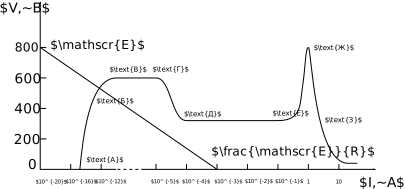
\includegraphics[width=0.7\textwidth]{Chapter_5/v5_6}
	\caption{ВАХ разряда в неоне при давлении 1 тор. Нагрузочная прямая проходит через область тлеющего разряда.}
	\figmark{Neon discharge VAC}
\end{figure}

Участок характеристики ГДЕЖ соответствует \important{тлеющему разряду}, причём его падающая часть ГД называется
\important{поднормальным тлеющим разрядом}, горизонтальная часть ДЕ~--- \important{нормальным тлеющим разрядом} и остальная часть
ЕЖ~--- \important{аномальным тлеющим разрядом}. Далее идёт падающий участок ЖЗ, который можно получить при маленьких
сопротивлениях и сильноточных источниках напряжения. Он соответствует переходу к \important{дуговому разряду}. Заметим, что
при больших давлениях газа (атмосферном и больше) после пробоя сразу устанавливается дуговой разряд.

Как уже говорилось выше, отличительной характеристикой таунсендовского разряда является однородность поля по длине
промежутка, что обусловлено малостью тока и отсутствием объёмных зарядов. Однако при большом токе разряда поле
перераспределяется после пробоя и почти полностью сосредотачивается у катода. Это обусловлено образованием у катода
положительного объёмного заряда за счёт ионного тока (электронный ток у катода мал по сравнению с ионным). Кроме того,
остальная часть газового промежутка переходит в состояние с высокой электропроводностью~--- образуется так называемый
положительный столб, замыкающий электрическую цепь. Таким образом, почти всё приложенное поле сосредоточено у катода на
участке, занятом объёмным зарядом. Следовательно, на этом участке, называемом катодным слоем, падает почти всё
приложенное к электродам напряжение~--- так называемое катодное падение потенциала. Оно примерно равно минимальному
напряжению пробоя для промежутка, длина которого равна толщине катодного слоя. Тем самым реализуются условия для
самоподдержания разряда (критерий Таунсенда) при гораздо меньших напряжениях, чем при однородном поле на всей длине
газового промежутка. Этот разряд, отличающийся от таунсендовского не только значительно большим током, но и главным
образом существенной неоднородностью приложенного поля~--- наличием катодного падения потенциала~--- и называется
тлеющим разрядом. Именно этим разрядом мы будем заниматься далее.
\todo[author = Andrew]{В картинке для нанесения некоторых обозначений был использован psfrag, который несовместим с pdf. Необходимо исправить изображение.}

\begin{figure}[h!]
	\centering
	\psfrag{-}[cc]{$-$}
	\psfrag{+}[cc]{$+$}
	\psfrag{r}[rb]{$\rho$}
	\psfrag{A}[bc]{$\rho=e(n_+-n_e)$}
	\psfrag{n}[rb]{$n$}
	\psfrag{B}[bc]{$n_+=n_e$}
	\psfrag{a}[cc]{$n_+$}
	\psfrag{b}{$n_e$}
	\psfrag{c}[cc]{$j_+$}
	\psfrag{d}[cb]{$j_e$}
	\psfrag{e}[cc]{$\leftarrow j$}
	\psfrag{f}[rb]{$|j|$}
	\psfrag{g}[rb]{$|E|$}
	\psfrag{E}[cb]{$E$}
	\psfrag{h}[rb]{$\phi$}
	\psfrag{i}{$V_а$}
	\psfrag{k}{$V_к$}
	\psfrag{l}[rb]{$I$}
	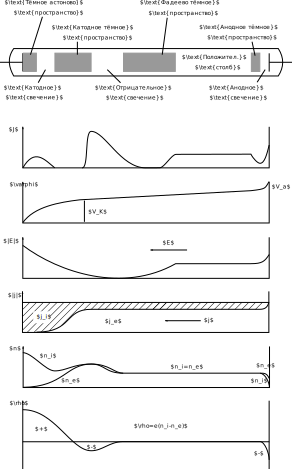
\includegraphics[width=0.5\textwidth]{Chapter_5/v5_7}
	\caption{Структура тлеющего разряда и распределение по длине основных характеризующих его величин}
	\figmark{Glow discharge}
\end{figure}

На рис.~\figref{Glow discharge} представлена качественная картина тлеющего разряда в длинной стеклянной трубке, а также приведены зависимости
основных величин, характеризующих разряд, от продольной координаты. Это интенсивность свечения, потенциал и
напряжённость электрического поля, электронный и ионный токи, электронная и ионная плотности и полная плотность
объёмного заряда.

Видно, что разряд состоит из ряда чередующихся светлых и тёмных поперечных полос. Поскольку все процессы в разряде
связаны со столкновениями электронов с атомами газа, расстояния от катода до этих полос определяются числом
укладывающихся на них длин пробега электронов. Поэтому характерные размеры полос увеличиваются с уменьшением давления.
Непосредственно к катоду прилегает узкое \important{астоново пространство,} затем идёт слой \important{катодного свечения}, а
затем~--- \important{тёмное катодное пространство}. Далее следует область \important{отрицательного свечения,} переходящая в
\important{тёмное фарадеево пространство}. За ним начинается светящийся \important{положительный столб}, заканчивающийся у анода
\important{тёмным анодным пространством}, переходящим на аноде в узкий слой \important{анодного свечения}.

Как правило, самой яркой бывает область отрицательного свечения, имеющего для воздуха голубоватый цвет, за что разряд и
получил своё название~--- тлеющий.

Качественно распределение свечения по длине разряда объясняется следующим образом.

Электроны, выбиваемые из катода приходящими на него ионами, имеют энергию, недостаточную для возбуждения атомов. Поэтому
слой у катода~--- тёмный (\important{астоново пространство}). Далее электроны набирают достаточную для этого энергию, и
возникает первый светящийся слой, \important{катодное свечение}. Затем энергия электронов становится настолько большой, что
они в основном ионизуют, а не возбуждают атомы. Так образуется \important{тёмное катодное пространство}, в котором происходит
основное размножение электронов и ионов. Рождающиеся ионы движутся к катоду, создавая большой \important{положительный
объёмный заряд}. В конце тёмного катодного пространства поля уже почти нет, оно перехвачено объёмным зарядом, зато
образовалось очень много движущихся к аноду сравнительно медленных электронов, которые снова возбуждают атомы. Так
начинается область \important{отрицательного свечения}. Далее электроны растрачивают свою энергию (поле слабое) и возбуждение
прекращается, а свечение переходит в \important{тёмное фарадеево пространство}.

В фарадеевом пространстве поле медленно нарастает до своего значения в положительном столбе, который можно рассматривать
просто как участок омического проводника с электронной проводимостью. Поскольку здесь непрерывно происходят столкновения
электронов с атомами, происходит их возбуждение, и положительный столб испускает свечение. У анода ионов нет, электроны
образуют \important{отрицательный объёмный заряд}, создаётся небольшое \important{анодное падение потенциала}, в котором электроны
набирают энергию и вызывают \important{анодное свечение}.

Все зависимости, показанные на рис.~\figref{Glow discharge}, подтверждают приведённое объяснение. Самым важным здесь является наличие зоны
положительного объёмного заряда и области сильного электрического поля у катода. Это и есть \important{катодный слой}, он
простирается от катода до начала области отрицательного свечения. Как уже говорилось выше, катодный слой~--- самая
важная часть тлеющего разряда, без него разряд существовать не может. Толщина катодного слоя и величина катодного падении
потенциала автоматически устанавливаются таким образом, чтобы выполнялись критерии самоподдержания разряда при минимуме
затрат энергии: это~--- минимальное для такого размера напряжение, примерно равное минимальному напряжению зажигания по
кривой Пашена. Это означает, что на создание одной электронно-ионной пары затрачивается минимальная энергия (равная так
называемой \important{константе Столетова}).

Особым свойством самоорганизации обладает \important{нормальный тлеющий разряд} , то есть разряд, напряжение на котором при
возрастании тока практически не меняется (горизонтальный участок ВАХ на рис.~\figref{Neon discharge VAC}). В нём ток может возрастать только
за счёт возрастания площади катодного пятна, а плотность тока остаётся неизменной. Качественно это можно объяснить тем,
что поскольку напряжение на катодном слое и его толщина задаются условием минимума на кривой Пашена, они почти не
меняются при заданном давлении газа. Следовательно, должна оставаться постоянной и плотность тока.

При полном заполнении катода дальнейшее увеличение тока будет возможно только за счёт повышения интенсивности ионизации
газа, что возможно только при повышении напряжения. Разряд при этом переходит в режим аномального тлеющего разряда
(участок ЕЖ на ВАХ). В аномальном разряде плотность тока выше, чем в нормальном.

Как это можно видеть на нижней кривой рис.~\figref{Glow discharge}, описывающей распределение объёмного заряда, между катодным слоем и анодом
образуется длинная (если трубка длинная) электронейтральная область, большая часть которой называется положительным
столбом. На рис.~\figref{Glow discharge} также видно, что в положительном столбе плотность электронов равна плотности ионов, ток в основном
переносится электронами, а вызывающее ток электрическое поле однородно по длине, как это имеет место в обычном омическом
проводнике. В соответствии со сказанным выше, такое состояние газа называется \important{плазмой}. Положительный столб
тлеющего газового разряда представляет собой пример \important{низкотемпературной слабоионизированной неравновесной плазмы}, поддерживаемой электрическим полем.

Состояние плазмы в положительном столбе совершенно не зависит от процессов в приэлектродных областях, а определяется
только процессами внутри него. Рождение и гибель электронов проходят на фоне их дрейфового движения от катода к аноду.
Потери электронов в столбе (за счёт диффузии к стенкам трубки, а также рекомбинации в объёме) должны компенсироваться
ионизацией. И всё-таки большая часть электронов, достигающих анода, поступает в столб извне (из катодного слоя), как это
происходит при токе через обычный проводник.

В нормальном тлеющем разряде в случае, когда потери электронов обусловлены диффузией, ВАХ положительного столба может
быть падающей. В этом случае падающей будет и ВАХ всего разряда, что подтверждает эксперимент: при увеличении тока
напряжение на разрядном промежутке не остаётся постоянным, как это должно быть для нормального тлеющего разряда, а
уменьшается.

Это объясняется нагревом газа. В центральной области газ нагревается сильнее, его концентрация понижается, длина пробега
электронов возрастает и они получают возможность набирать энергию, необходимую для ионизации, при меньшем поле, чем до
нагрева. Следовательно, напряжение, необходимое для поддержания такого тока, понижается.

Случайные локальные перегревы, а также другие процессы, приводящие к появлению отрицательного дифференциального
сопротивления, могут быть причиной развития различных \important{неустойчивостей}. Механизм, типа описанного выше, может
вызвать стягивание разряда в токовый шнур (\important{контракция}). Этим объясняется переход аномального разряда в дуговой:
катодное пятно уменьшается настолько, что катод в этом месте накаляется и начинается термоэмиссия. Другие неустойчивости
ведут к образованию в положительном столбе поперечных слоёв, или \important{страт}, которые, как правило, движутся в
продольном направлении.

\labsection{Высокочастотный нагрев плазмы}

Ионизацию в плазме можно создать и с помощью высокочастотного электромагнитного поля. Существуют различные способы
введения высокочастотного поля в разрядный объём. Один из них основан на электромагнитной индукции: через
катушку-соленоид, в которую вставлена диэлектрическая (например, стеклянная) газоразрядная камера, пропускается ток
высокой частоты, и внутри катушки индуцируется вихревое электрическое поле. Силовые линии этого поля, а вместе с ними и
линии тока в газоразрядной камере образуют замкнутые круговые линии. Такой разряд называется кольцевым, индукционным или
разрядом H-типа, что указывает на определяющую роль магнитного поля.

Другой способ возбуждения заключается в том, что высокочастотное напряжение подаётся на электроды, которые могут
непосредственно соприкасаться с разрядной плазмой или быть изолированы от неё диэлектриками (стенками разрядной камеры).
Система двух электродов ведёт себя по отношению к переменному напряжению как конденсатор, поэтому такие разряды
называются ёмкостными или разрядами E-типа.

Высокочастотные разряды успешно используются в технике. Индукционные разряды применяются в безэлектродных генераторах
плотной низкотемпературной плазмы (в плазмотронах), применяемых, например, для плазмохимического производства чистых
веществ. Разряды ёмкостного типа применяются в мощных газоразрядных лазерах.

Исследуем электрический пробой в высокочастотном поле. Начнём с исследования движения электрона при низком давлении
газа, когда столкновения с молекулами происходят редко. Движение электрона в однородном переменном электрическом поле
описывается уравнением
\begin{equation*}
	m_e\frac{d^2x}{dt^2}=-eE_0\sin\omega t,
\end{equation*}
где $E_0$~--- амплитуда электрического поля. Интегрируя это уравнение, получим
\begin{equation*}
	v=v_0+\frac{eE_0}{\omega m_e}\cos\omega t,
\end{equation*}
где $v_0$~--- скорость электрона в момент $t=0$.

Мы видим, что скорость электрона периодически увеличивается и уменьшается, но в среднем энергии от поля электрон не
получает. Так обстоит дело, пока вакуум достаточно высок. При увеличении давления всё чаще происходят соударения
электронов с молекулами газа, однако медленные электроны не могут ионизировать молекулы и соударяются с ними упруго.

Чтобы понять, как возникает пробой, исследуем, что происходит при упругом соударении электрона с молекулами газа. Как
уже отмечалось, при таких соударениях электрон почти не теряет кинетической энергии, однако направление его скорости
претерпевает существенные изменения и может вновь совпасть с изменившимся направлением электрического поля. В этом
случае электрон при дальнейшем движении не возвращает полю энергию, а вновь её получает. Часть электронов может поэтому
заметно ускоряться высокочастотным полем. Увеличение энергии электрона продолжается до тех пор, пока она не станет
достаточной для ионизации газа. Затем процесс повторяется: при упругих столкновениях с молекулами газа часть электронов
в электрическом поле ускоряется, вследствие чего происходят новые акты ионизации. Таким образом, в газе накапливаются
электроны и ионы. По мере увеличения их концентрации возрастает роль процессов рекомбинации. В результате действия этих
двух факторов~--- ионизации и рекомбинации~--- устанавливается стационарная плазма. Её концентрация и температура
зависят от сорта газа, его давления, а также от частоты и амплитуды высокочастотного поля.

\begin{lab:questions}

\item Назовите различные виды плазм в лаборатории, приложениях и природе. Параметры плазмы.

\item Что такое дебаевский радиус экранирования?

\item Дайте строгое определение понятия \important{плазма}.

\item Что такое плазменная частота? Выведите формулу для плазменной частоты. Какие процессы в плазме характеризуются плазменной частотой?

\item Чем определяется потенциал зонда, погружённого в плазму?

\item Чем определяется зондовый ток насыщения для одиночного зонда? Для двойного зонда?

\item Перечислите виды газового разряда.

\item Что такое вольт-амперная характеристика газового разряда?

\item Приведите основные параметры нормального тлеющего разряда. Является ли он источником стацтонарной равновесной плазмы?

\item Опишите основной механизм зажигания тлеющего разряда.

\item Каков механизм зажигания разряда в высокочастотном поле?

\end{lab:questions}


\begin{lab:literature}

\item \emph{Сивухин Д.В.} Общий курс физики. Т.~III. Электричество.~--- М.: Наука, 1983. Гл. IX.

\item \emph{Кингсеп А.С.} Элементы физики плазмы: Учебно-методическое пособие. ~--- М:МФТИ 1985.

\item \emph{Райзер Ю.П.} Физика газового разряда.~--- Долгопрудный: Издательский Дом Интеллект, 2009.

\item \emph{Чен Ф.} Введение в физику плазмы. Перевод с английского ~--- М.: Мир, 1987.

\item \emph{Князев Б.А.} Низкотемпературная плазма и газовый разряд: Учебное пособие/ Новосибирский государственный университет. ~--- Новосибирск, 2003.
\end{lab:literature}